\subsection{Introduction}
\subsubsection{Purpose}
Rockwell Collins currently develops their vision systems on Field Programmable Gate Arrays, making the time from design to product very long.  Rockwell Collins is considering using Single Board Computers as a way to speed up this cycle.
Our goal is to provide a proof of concept for a vision system on a Single Board Computer for Rockwell Collins. This proof of concept should help Rockwell Collins measure the practicality of Single Board Computers for vision systems.\\

\subsubsection{Scope}
Development will be limited to the Jetson TK1 or Jetson TX1. Evaluation of hardware platforms other than the TK1 and TX1 will be a stretch goal. In which case, these boards will serve as the base unit for comparison. Software shall interface to a minimum of 2 cameras, receive video, and display it on a monitor while logging metrics. Metrics will be frames per second and operations per second.\\

\subsubsection{Definitions}
\begin{description}[leftmargin=2cm,labelindent=2cm]
	\item [SBC] Single board computer
	\item [RC] Rockwell Collins
	\item [FPS] Frames per second
	\item [FPGA] Field-programmable gate array
	\item [USB] Universal serial bus
	\item [PoC] Proof of concept
	\item [SVS] Simple vision system\\
\end{description}

\subsubsection{References}
Carlo Tiana, Airborne Vision Systems Expert at Rockwell Collins
Weston Lahr, Senior Software Engineer at Rockwell Collins,
Jetson TK1 Embedded Hardware, NVIDIA\\

\subsubsection{Assumptions and Constraints}
We're assuming that either Jetson model can handle some sort of camera vision system. From initial investigations it appears that the Jetson TX1 is a likely candidate to support our project goals.

\subsection{Overall Description}
This section will give a bird's eye view of the project, outlining the major features and their purpose.\\
\subsubsection{Product Perspective}
  \paragraph{System Interfaces}
  Linux, Jetson Distro
  \paragraph{User Interfaces}
  While using our deliverable, the user should be able to view output image from the Jetson.
  \paragraph{Software Interfaces}
  Our deliverable should be a demonstrate of the Jetson's video output, charts that display capability performance, information about the complexity and amount of video processing operations. A stretch goal would include to have the same output of the software running on a second screen.
  \paragraph{Hardware Interfaces}
  We must choose an interface between our program and the chosen camera attached to the Jetson SBC. We must also interface with the relative camera processing systems on the Jetson.
  \paragraph{Communication Interfaces}
  We will communicate with at least two different camera streams, from two separate cameras attached to our SBC.\\
  
\subsubsection{Product Functions}
The delivered demonstration should accurately demonstrate the performance limitations of the Jetson TK1 or TX1. Should the timeframe allow, we are to continue investigating other SBCs and providing a similar overview of other researched SBCs.\\

\subsubsection{User Characteristics}
Our users will be RC developers, looking to implement a given filter for vision processing platforms.\\

\subsubsection{Constraints}
Our deliverable must run on either the Jetson TK1 or Jetson TX1, and should simply test the Jetson's capabilities. We will use 1080p cameras.\\

\subsubsection{Assumptions and Dependencies}
We are assuming that the Jetson can at least handle some level of video processing.We are also going to rely on libraries and the operating system provided by Nvidia for the Jetson.\\

\subsubsection{Stretch Goal Timeline}
Stretch goals defined throughout this document may be delayed until all other requirements are finished and are not required to be in the deliverable at any point.

\subsection{Specific Requirements}
This section will outline some of the more specific parts of the project along with exact requirements that the deliverable should meet.\\

\subsubsection{External Interfaces}
\begin{description}[leftmargin=2cm,labelindent=2cm]
	\item [Two 1080p Cameras] These will be used to transfer video data to the Jetson to be processed and displayed on a monitor.
	\item [Monitor] Any monitor able to adequately display the output of the chosen SBC for the purposes of evaluation. 
	\item [Jetson] Should be able to read and process video data and stream it out to a monitor.\\
\end{description}

\subsubsection{Functions}
The system shall take input from the cameras and perform as much video processing on it as possible before dipping under the 30 fps minimum.
If the system can't handle 30fps without any extra video processing, it should simply be displayed at the fastest fps possible.\\

\subsubsection{Performance Requirements}
The system should support at least 2 cameras with a stretch goal of 3 cameras.
The system should support video output on one monitor, and if possible the video should be displayed at 30fps.\\

\subsubsection{Design Constraints}
Since this is a proof of concept, the only real design constraint is that it should be able to correctly assess and demonstrate the hardware limitations of the Jetson SBC.\\

\subsubsection{Maintainability}
Maintainability, outside of our timeframe, is a low-priority requirement as we are only delivering a proof of concept for the capabilities of our SBC.\\

\subsubsection{Portability}
Our software should give some idea of how similar code would perform on other platforms, even though the PoC itself does not have to be portable. The same goes for the camera and monitor.In order to help our stretch goal of evaluating a second SBC, it would help if the code, cameras, and monitor were all collectively portable to the second platform.\\

\subsection{Stretch Goals}
Some stretch goals were listed throughout the requirements. One purpose of the stretch goals is to further increase the effectiveness of the proof of concept. These added goals further stress the limitations of the Jetson TK1 or TX1, to further expand the capabilities of these SBC. A few other stretch goals not mention above would be implementing the same system on a similar SBC, and comparing that with the Jetson TK1 or TX1, or implementing object tracking as a video processing operation to test performance of the SBCs.\\

\subsection{Gantt Chart}
\begin{figure}[H] 
\centering
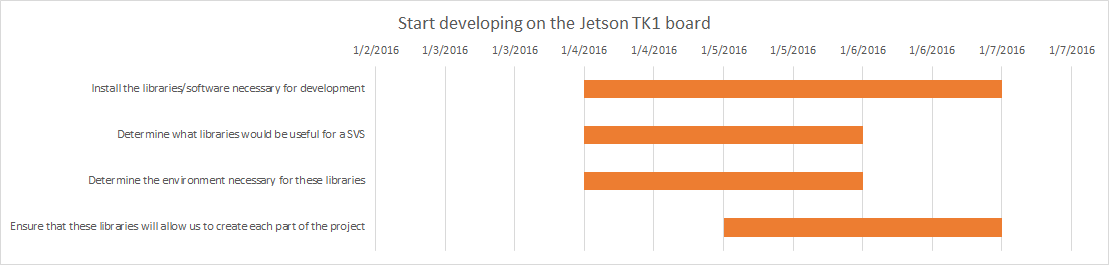
\includegraphics[width=1.0\textwidth,natwidth=1210,natheight=642]{gantt/original/starting.png}  
\end{figure}
\begin{figure}[H] 
\centering
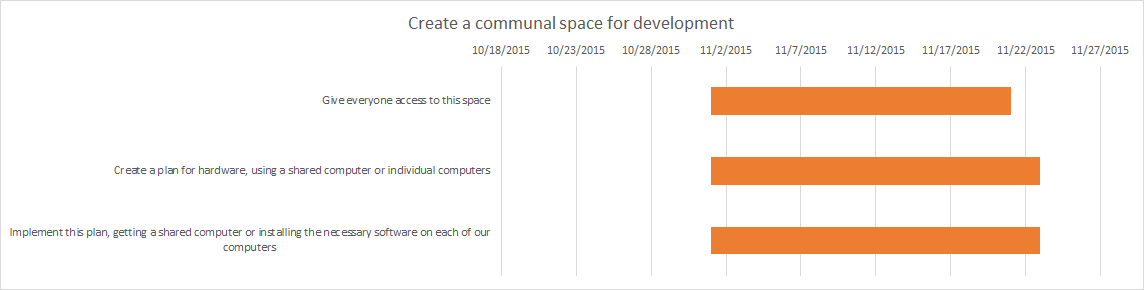
\includegraphics[width=1.0\textwidth,natwidth=1210,natheight=642]{gantt/original/communal.png}  
\end{figure}
\begin{figure}[H] 
\centering
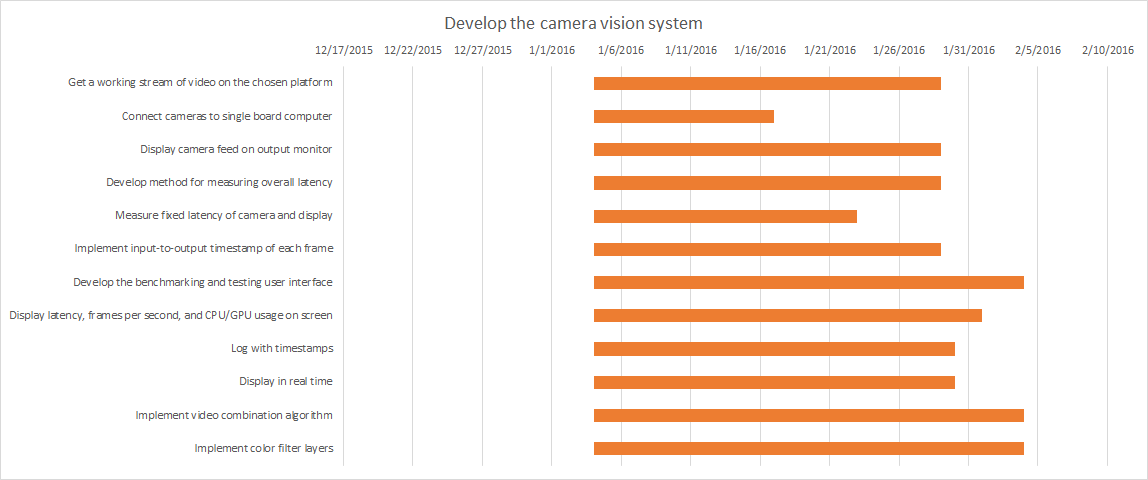
\includegraphics[width=1.0\textwidth,natwidth=1210,natheight=642]{gantt/original/develop.png}  
\end{figure}
\begin{figure}[H] 
\centering
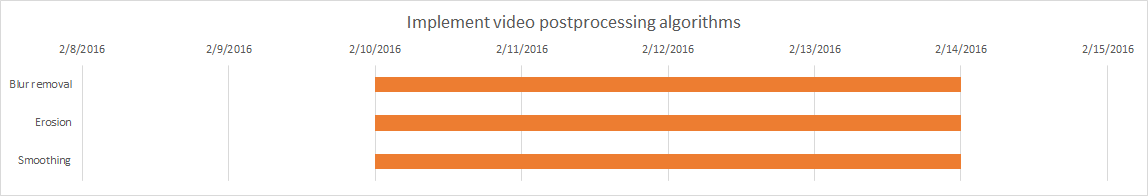
\includegraphics[width=1.0\textwidth,natwidth=1210,natheight=642]{gantt/original/algos.png}  
\end{figure}
\begin{figure}[H] 
\centering
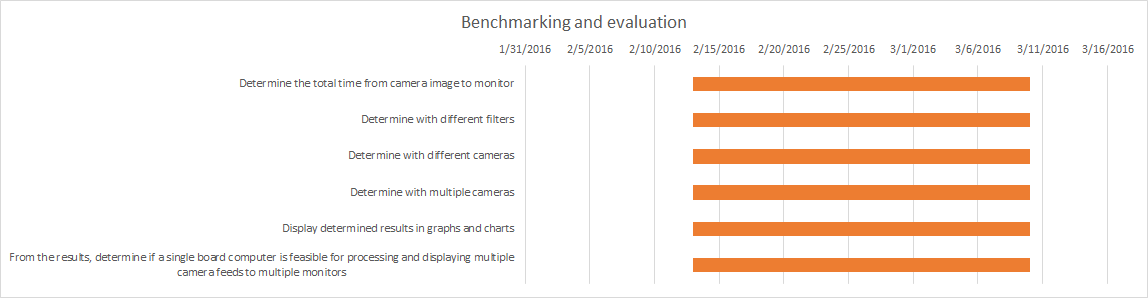
\includegraphics[width=1.0\textwidth,natwidth=1210,natheight=642]{gantt/original/eval.png}  
\end{figure}
\begin{figure}[H] 
\centering
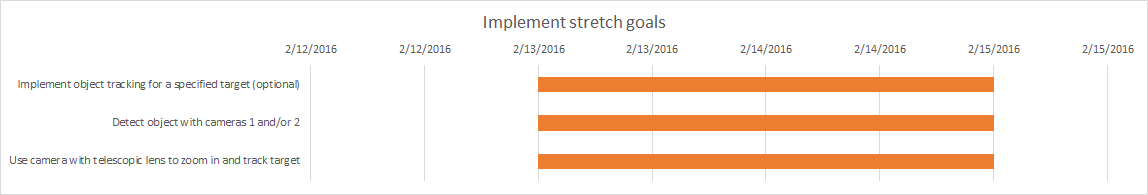
\includegraphics[width=1.0\textwidth,natwidth=1210,natheight=642]{gantt/original/stretch_goals.png}  
\end{figure}

